\documentclass[a4paper]{beamer}

%\usepackage[T1]{fontenc}
\usepackage[utf8]{inputenc}
\usepackage{bbm}
\usepackage{lmodern,charter,environ}
\usepackage{listings}
\usepackage{xcolor}
\usepackage{graphicx}

\definecolor{yellow-creme-brulee}{rgb}{0.99,0.87,0.50}
\definecolor{pink-froly}{rgb}{1,0.23,0.35}
\definecolor{tuft-bush}{rgb}{0.99,0.81,0.69}
\definecolor{blue-portage}{rgb}{0.32,0.45,0.81}
\definecolor{blue-marguerite}{rgb}{0.30,0.13,0.65}
\definecolor{blue-oxford}{rgb}{0.21,0.27,0.34}
\definecolor{green-de-york}{rgb}{0.33,0.75,0.44}
\definecolor{green-pea}{rgb}{0,0.33,0.25}
\definecolor{orange-vivid-tangerine}{rgb}{0.98,0.47,0.31}
\definecolor{dark-grey}{rgb}{0.53,0.54,0.54}
\definecolor{bright-grey}{rgb}{0.85,0.85,0.84}

\lstdefinelanguage{Terminal}{
    moredelim=[is][\color{bright-grey}]{\$@}{@\$},
} %
\lstdefinelanguage{Nix}{
    keywords=[1]{
      if,
      then,
      else,
    },
    keywords=[2]{
      let,
      rec,
      in
    },
    keywords=[3]{
      true,
      false,
      null
    },
    sensitive=true, % keywords are case-sensitive
    morecomment=[l]{\#}, % l is for line comment
    morestring=[b]", % defines that strings are enclosed in double quotes
    morestring=[b]'',
    moredelim=[is][\color{bright-grey}]{\$@}{@\$},
} %
\lstdefinelanguage{Nickel}{
    keywords=[1]{
      if,
      then,
      else,
      switch,
    },
    keywords=[2]{
      let,
      rec,
      fun,
      in
    },
    keywords=[3]{
      Num,
      Bool,
      Str,
      List,
      forall,
    },
    keywords=[4]{
      true,
      false,
      null
    },
    keywords=[5]{
      doc,
      default,
    },
    sensitive=true, % keywords are case-sensitive
    morecomment=[l]{//}, % l is for line comment
    morecomment=**[is][\color{dark-grey}]{\$}{\$},
    morestring=[b]", % defines that strings are enclosed in double quotes
    morestring=[s]{m\#"}{"\#m},
    moredelim=[is][\color{bright-grey}]{\$}{\$},
} %

\colorlet{punct}{red!60!black}
\definecolor{background}{HTML}{EEEEEE}
\definecolor{delim}{RGB}{20,105,176}
\colorlet{numb}{magenta!60!black}

\lstdefinelanguage{json}{
    basicstyle=\normalfont\ttfamily,
    numbers=left,
    numberstyle=\scriptsize,
    stepnumber=1,
    numbersep=8pt,
    showstringspaces=false,
    breaklines=true,
    literate=
     *{0}{{{\color{numb}0}}}{1}
      {1}{{{\color{numb}1}}}{1}
      {2}{{{\color{numb}2}}}{1}
      {3}{{{\color{numb}3}}}{1}
      {4}{{{\color{numb}4}}}{1}
      {5}{{{\color{numb}5}}}{1}
      {6}{{{\color{numb}6}}}{1}
      {7}{{{\color{numb}7}}}{1}
      {8}{{{\color{numb}8}}}{1}
      {9}{{{\color{numb}9}}}{1}
      {:}{{{\color{punct}{:}}}}{1}
      {,}{{{\color{punct}{,}}}}{1}
      {\{}{{{\color{delim}{\{}}}}{1}
      {\}}{{{\color{delim}{\}}}}}{1}
      {[}{{{\color{delim}{[}}}}{1}
      {]}{{{\color{delim}{]}}}}{1},
    moredelim=[is][\color{bright-grey}]{\$}{\$},
}

\lstdefinestyle{Terminal}{
  language={Terminal},
  backgroundcolor = \color{bright-grey},
  basicstyle=\small\ttfamily, % Global Code Style
  captionpos=b, % Position of the Caption (t for top, b for bottom)
  extendedchars=true, % Allows 256 instead of 128 ASCII characters
  tabsize=2, % number of spaces indented when discovering a tab
  columns=fixed, % make all characters equal width
  keepspaces=true, % does not ignore spaces to fit width, convert tabs to spaces
  showstringspaces=false, % lets spaces in strings appear as real spaces
  breaklines=true, % wrap lines if they don't fit
  frame=trbl, % draw a frame at the top, right, left and bottom of the listing
  framesep=4pt, % quarter circle size of the round corners
  numbers=none, % show line numbers at the left
}

\lstset{
  language={Nix},
  basicstyle=\small\ttfamily, % Global Code Style
  captionpos=b, % Position of the Caption (t for top, b for bottom)
  extendedchars=true, % Allows 256 instead of 128 ASCII characters
  tabsize=2, % number of spaces indented when discovering a tab
  columns=fixed, % make all characters equal width
  keepspaces=true, % does not ignore spaces to fit width, convert tabs to spaces
  showstringspaces=false, % lets spaces in strings appear as real spaces
  breaklines=true, % wrap lines if they don't fit
  frame=trbl, % draw a frame at the top, right, left and bottom of the listing
  frameround=tttt, % make the frame round at all four corners
  framesep=4pt, % quarter circle size of the round corners
  numbers=left, % show line numbers at the left
  numberstyle=\tiny\ttfamily, % style of the line numbers
  commentstyle=\color{dark-grey}, % style of comments
  keywordstyle=[1]\color{blue-portage}, % style of keywords
  keywordstyle=[2]\color{orange-vivid-tangerine}, % style of keywords
  keywordstyle=[3]\color{blue-portage}, % style of keywords
  stringstyle=\color{blue-marguerite}, % style of strings
}

\lstset{
  language={Nickel},
  basicstyle=\small\ttfamily, % Global Code Style
  captionpos=b, % Position of the Caption (t for top, b for bottom)
  extendedchars=true, % Allows 256 instead of 128 ASCII characters
  tabsize=2, % number of spaces indented when discovering a tab
  columns=fixed, % make all characters equal width
  keepspaces=true, % does not ignore spaces to fit width, convert tabs to spaces
  showstringspaces=false, % lets spaces in strings appear as real spaces
  breaklines=true, % wrap lines if they don't fit
  frame=trbl, % draw a frame at the top, right, left and bottom of the listing
  frameround=tttt, % make the frame round at all four corners
  framesep=4pt, % quarter circle size of the round corners
  numbers=left, % show line numbers at the left
  numberstyle=\tiny\ttfamily\color{green-de-york}, % style of the line numbers
  commentstyle=\color{dark-grey}, % style of comments
  keywordstyle=[1]\color{blue-portage}, % style of keywords
  keywordstyle=[2]\color{orange-vivid-tangerine}, % style of keywords
  keywordstyle=[3]\color{blue-portage}, % style of keywords
  keywordstyle=[4]\color{green-pea}, % style of keywords
  keywordstyle=[5]\color{pink-froly}, % style of keywords
  stringstyle=\color{blue-marguerite}, % style of strings
}

\newcommand{\couleur}[2]{{\color{#1}{#2}}}

\usetheme{metropolis}

\setbeamercolor{progress bar}{fg=orange-vivid-tangerine}
\setbeamercolor{alerted text}{fg=orange-vivid-tangerine}
\setbeamercolor{example text}{fg=green-pea}
\setbeamercolor{normal text}{fg=blue-oxford}
\setbeamercolor{frametitle}{bg=blue-oxford}

\author{Yann Hamdaoui}
\title{A Tale of Nix and Nickel}
\subtitle{YOW! Lambda Jam}
\date{May 5, 2021}
% Hacky way to put the logo below, and not above
\titlegraphic{%
  \begin{picture}(0,0)
    \put(57,-190){\makebox(0,0)[rt]{
\includegraphics[width=2cm]{img/logo-tweag.pdf}}}
  \end{picture}}

\begin{document}

% \addtobeamertemplate{footline}{\insertframenumber/\inserttotalframenumber}

\newenvironment{frcseries}{\fontfamily{frc}\selectfont}{}
\newcommand{\textfrc}[1]{{\frcseries#1}}

\begin{frame}
\titlepage
\end{frame}

\section{Introduction}

\subsection{Cautionary tales}

\begin{frame}{A cautionnary tale}
Once upon a time...
\end{frame}

\subsection{Reproducibility}

\begin{frame}{Reproducibility}
    \begin{center}
        
\includegraphics[width=0.6\textwidth]{img/works-on-my-machine.pdf}
    \end{center}

    \vspace{10pt}

    \uncover<2-> {
    \begin{alertblock}{Reproducibility}
    \begin{enumerate}
        \item<3-> Concrete and widespread
        \item<4-> Mainstream tools do don't this well
    \end{enumerate}
    \end{alertblock}
}
\end{frame}

\begin{frame}{The problem}
    \begin{center}
        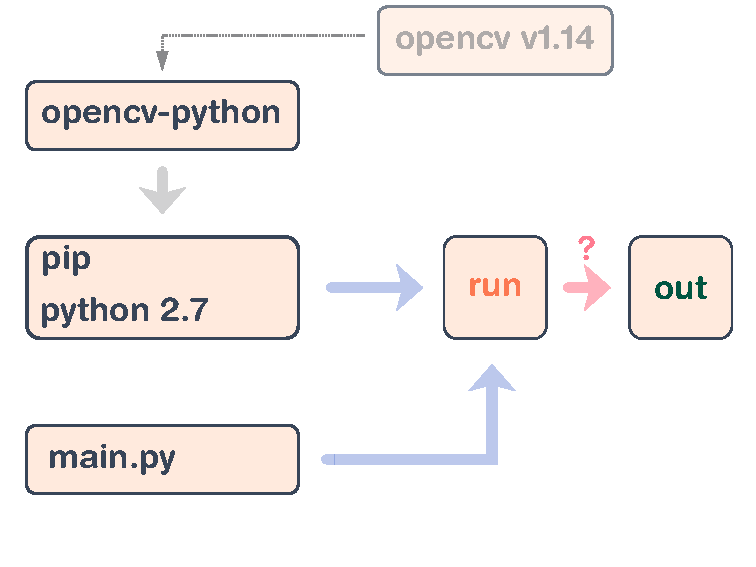
\includegraphics[width=0.95\textwidth]{img/schema-build.pdf}
    \end{center}
\end{frame}

\begin{frame}{Looks familiar?}
    \only<1> {
        \begin{center}
            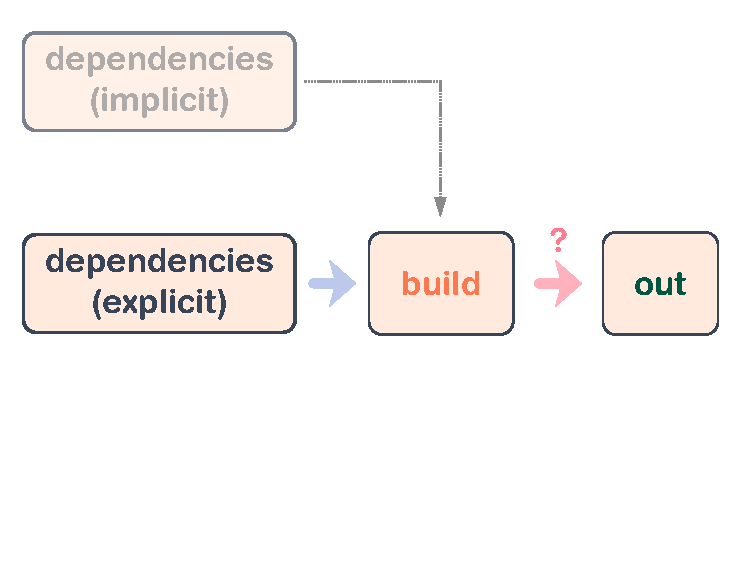
\includegraphics[width=0.95\textwidth]{img/schema-build-simplified.pdf}
        \end{center}
    }
    \only<2> {
        \begin{center}
            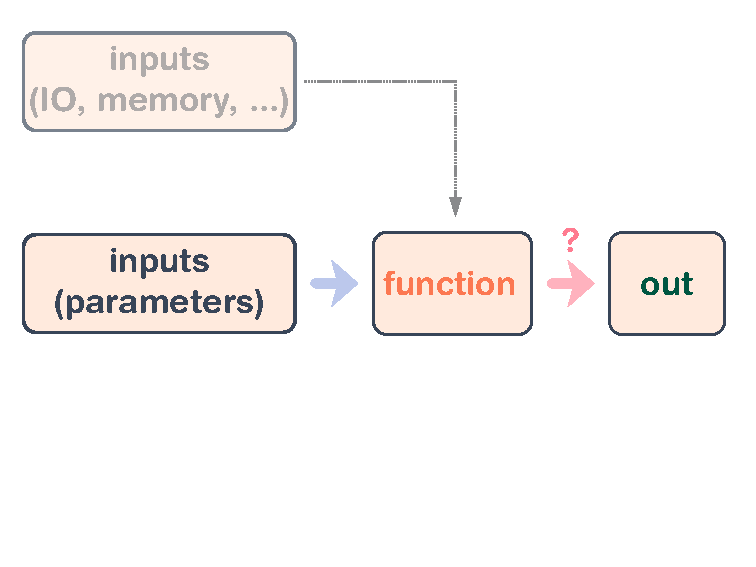
\includegraphics[width=0.95\textwidth]{img/schema-build-functional.pdf}
        \end{center}
    }
\end{frame}

\begin{frame}{Functional approach to reproducibility}
    \begin{center}
        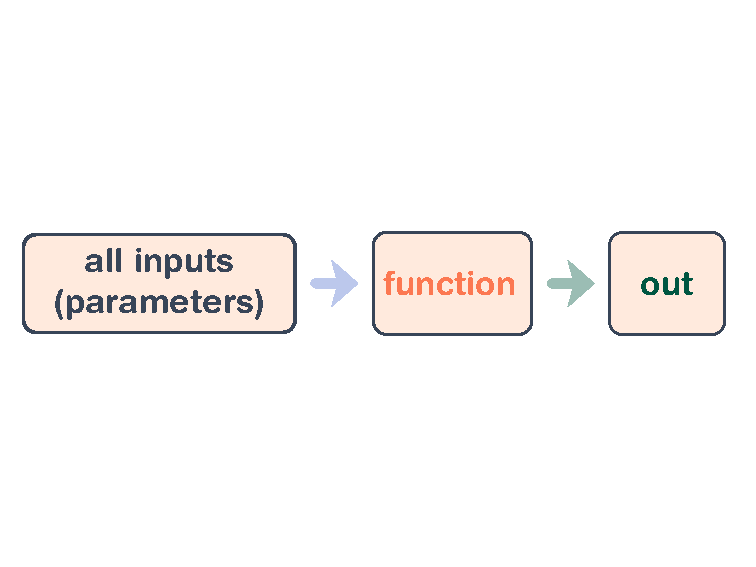
\includegraphics[width=0.95\textwidth]{img/schema-build-functional-correct.pdf}
    \end{center}
\end{frame}

\section{Nix: the functional package manager}

\begin{frame}
    \only<1> {
        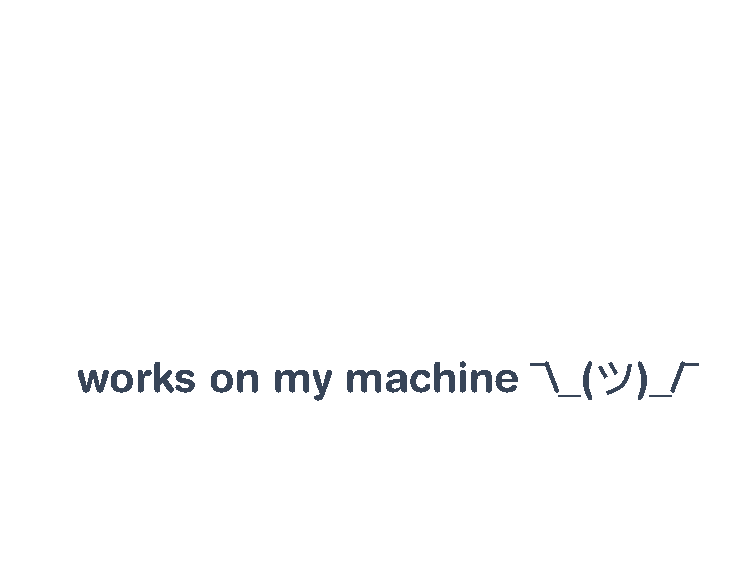
\includegraphics[width=0.95\textwidth]{img/schema-nix-motto-pre.pdf}
    }
    \only<2> {
        
\includegraphics[width=0.95\textwidth]{img/schema-nix-motto.pdf}
    }
\end{frame}

\begin{frame}
    \begin{block}{Principles}
        \begin{enumerate}
            \item<2-> \couleur{blue-portage}{Describe} a package and its
                dependencies in full
         \end{enumerate}
    \end{block}
\end{frame}

\begin{frame}[fragile]{Describing}
\begin{lstlisting}[language=Nix,title={gh-from-shoe-1-0.drv}]
Derive(
  [("out","/nix/store/qya..-gh-from-shoe","","")],
  [
    ("/nix/store/ae4..-python-2-7-10.drv",
      ["out"]),
    ("/nix/store/78f..-opencv-1-14.drv",
      ["out"]),
    ...
  ["/nix/store/9kr..-default-builder.sh"],
  "x86_64-linux",
  ...
\end{lstlisting}
\end{frame}

\begin{frame}
    \begin{block}{Principles}
        \begin{enumerate}
            \item \couleur{dark-grey}{Describe a package and its
                dependencies in full}
            \item
                \couleur{blue-portage}{Build} it in isolation
        \end{enumerate}
    \end{block}
\end{frame}

\begin{frame}{Building}
    \couleur{green-pea}{gh-from-shoe-1.0\$}\ \couleur{blue-marguerite}{nix build}
    \begin{enumerate}
        \item Pull and build dependencies\\
            (\lstinline+opencv-1-14+, \lstinline+python-2-7-10+, \ldots)
        \item Create an isolated environment.
        \item Run the builder.
    \end{enumerate}
\end{frame}

\begin{frame}
    \begin{block}{Principles}
        \begin{enumerate}
            \item
                \couleur{dark-grey}{Describe a package and its
                dependencies in full}
            \item
                \couleur{dark-grey}{Build it in isolation}
            \item
                Put the result in the
                \couleur{orange-vivid-tangerine}{store}
        \end{enumerate}
    \end{block}
\end{frame}

\begin{frame}{Storing}
    \only<1> {
\begin{center}
    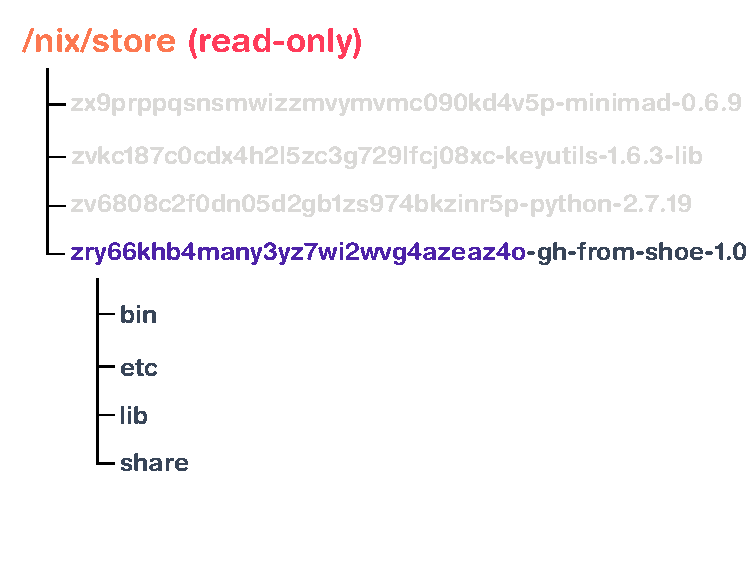
\includegraphics[width=0.95\textwidth]{img/schema-nix-store.pdf}
\end{center}
 }
    \only<2> {
\begin{center}
    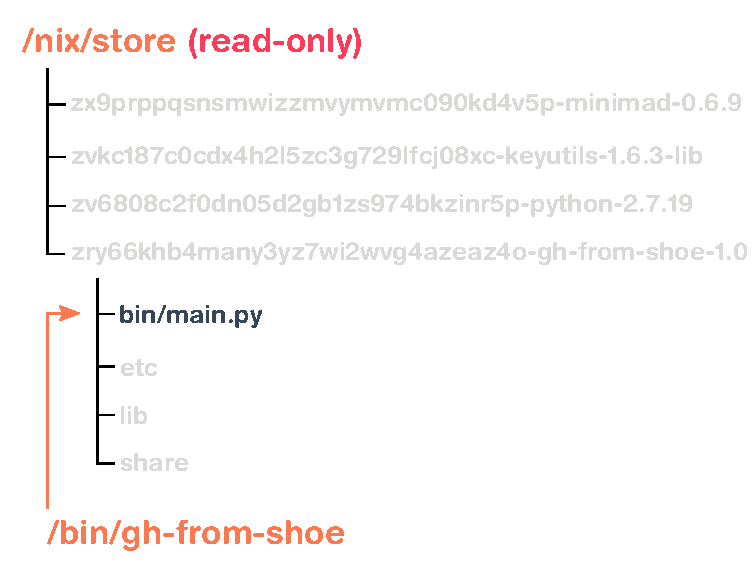
\includegraphics[width=0.95\textwidth]{img/schema-nix-store-link.pdf}
\end{center}
}
\end{frame}

\begin{frame}{Sharing}
\begin{center}
    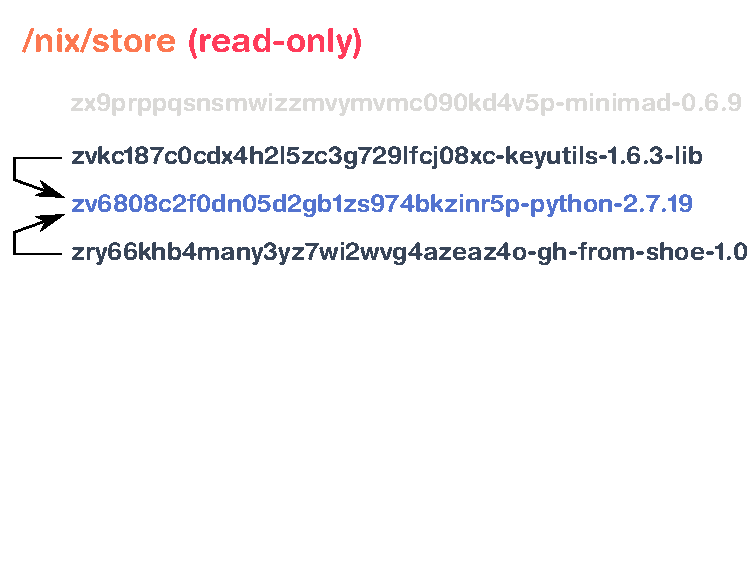
\includegraphics[width=0.95\textwidth]{img/schema-nix-store-sharing.pdf}
\end{center}
\end{frame}

\begin{frame}
    \begin{block}{Principles}
        \begin{enumerate}
            \item \couleur{dark-grey}{Describe a package and its
                dependencies in full}
            \item \couleur{dark-grey}{Build it in isolation}
            \item \couleur{dark-grey}{Put the result in the store}
            % \item<5> \couleur{blue-portage}{Profit}
            \item<1->
                \only<1> { \couleur{blue-portage}{Profit!} }
                \only<2-> { \couleur{dark-grey}{Profit!} }
            \item<2-> \couleur{blue-portage}{Clean}
        \end{enumerate}
    \end{block}
\end{frame}

\begin{frame}{Cleaning}
    \only<1> {
        \begin{center}
            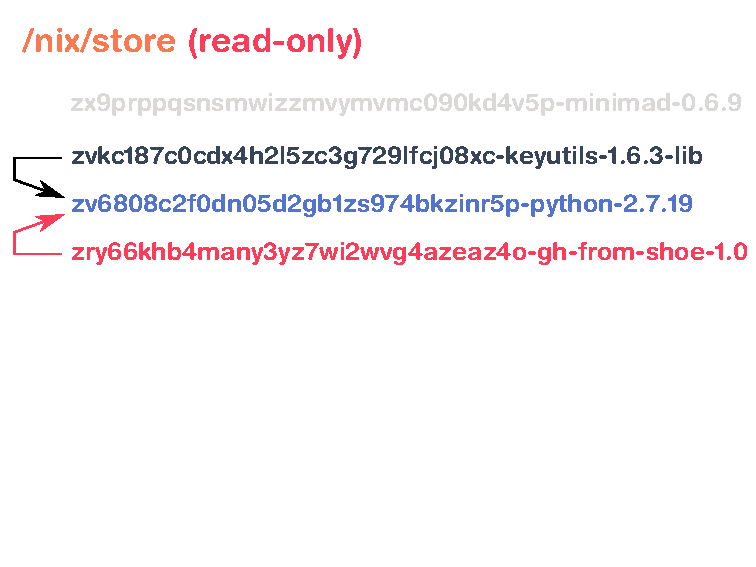
\includegraphics[width=0.95\textwidth]{img/schema-nix-store-cleaning-1.pdf}
        \end{center}
    }
    \only<2> {
        \begin{center}
            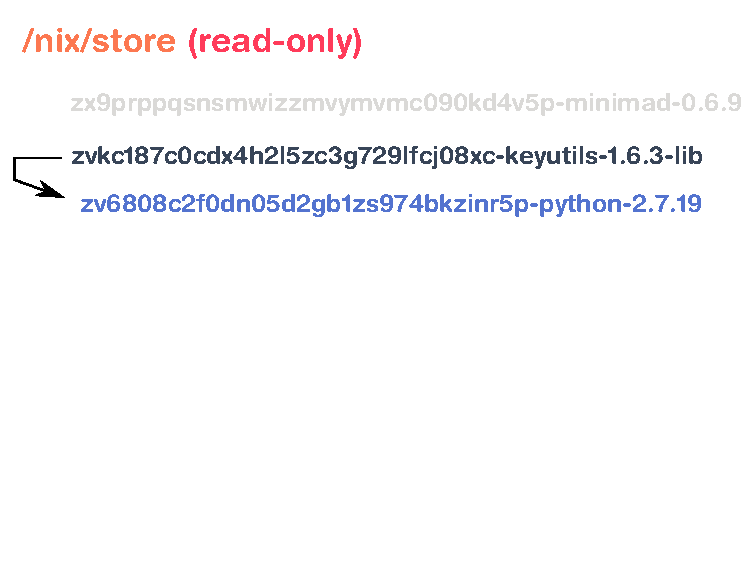
\includegraphics[width=0.95\textwidth]{img/schema-nix-store-cleaning-2.pdf}
        \end{center}
    }
    \only<3> {
        \begin{center}
            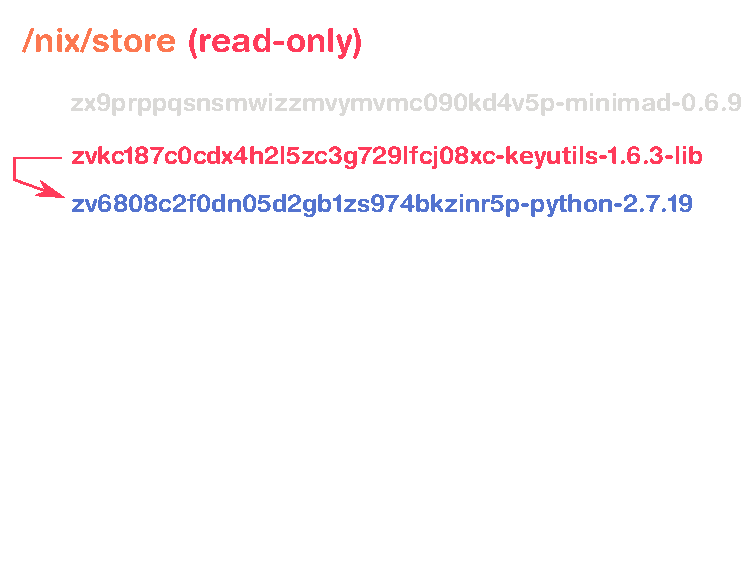
\includegraphics[width=0.95\textwidth]{img/schema-nix-store-cleaning-3.pdf}
        \end{center}
    }
    \only<4> {
        \begin{center}
            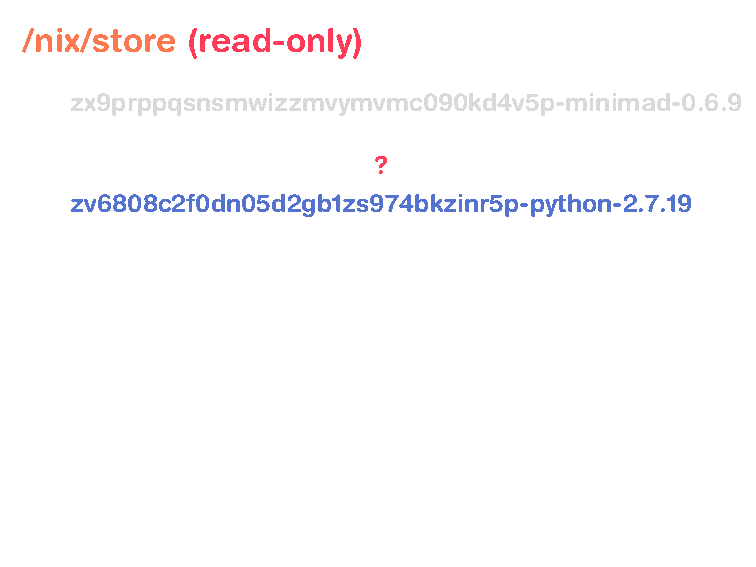
\includegraphics[width=0.95\textwidth]{img/schema-nix-store-cleaning-4.pdf}
        \end{center}
     }

    \only<5> {
        \begin{center}
            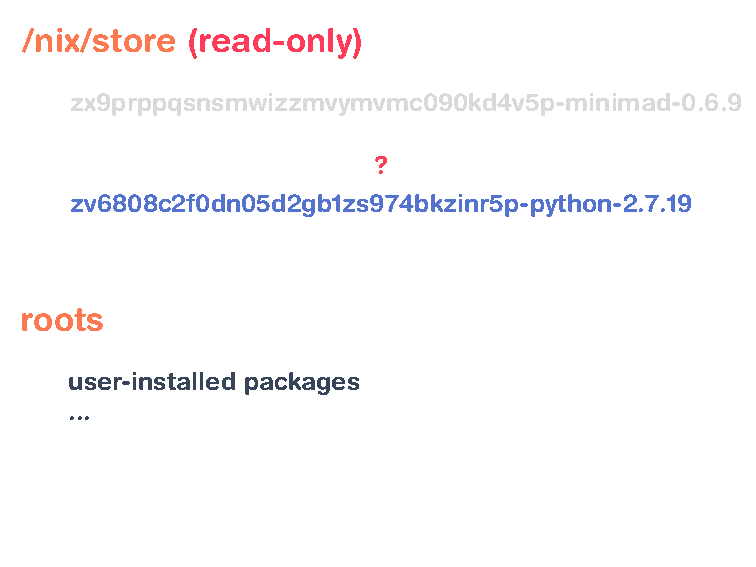
\includegraphics[width=0.95\textwidth]{img/schema-nix-store-cleaning-roots.pdf}
        \end{center}
    }
    \only<6> {
        \begin{center}
            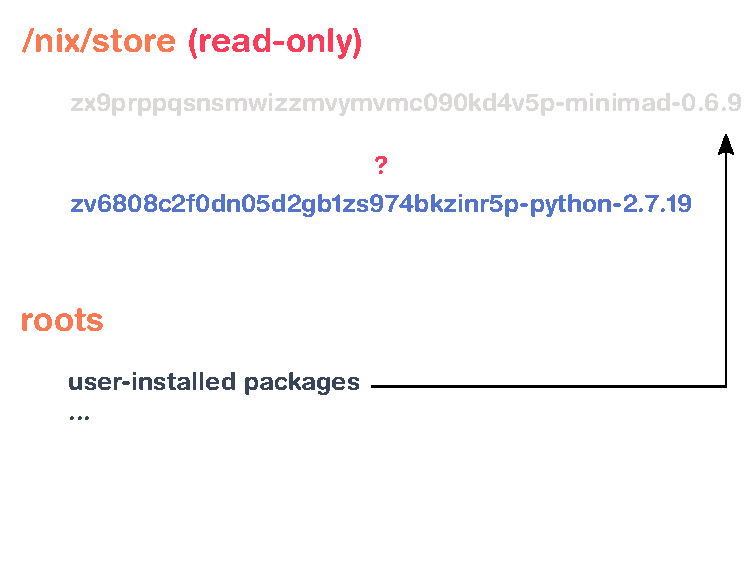
\includegraphics[width=0.95\textwidth]{img/schema-nix-store-gc-1.pdf}
        \end{center}
    }
    \only<7> {
        \begin{center}
            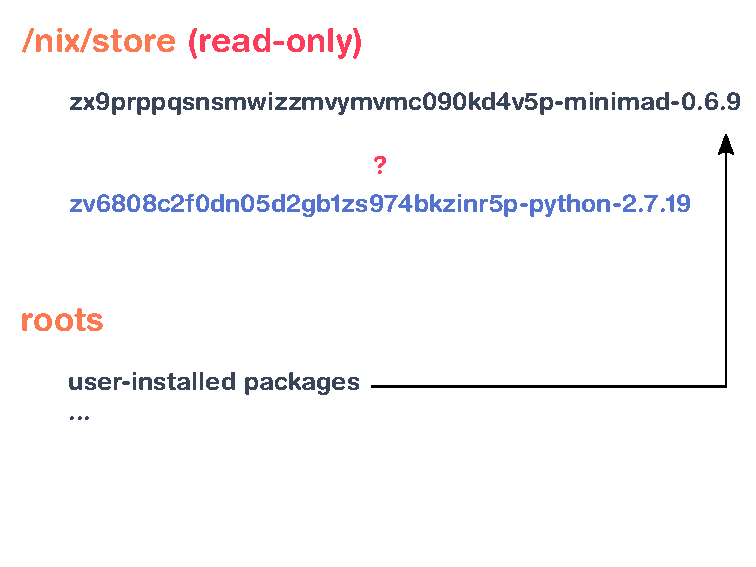
\includegraphics[width=0.95\textwidth]{img/schema-nix-store-gc-2.pdf}
        \end{center}
    }
    \only<8> {
        \begin{center}
            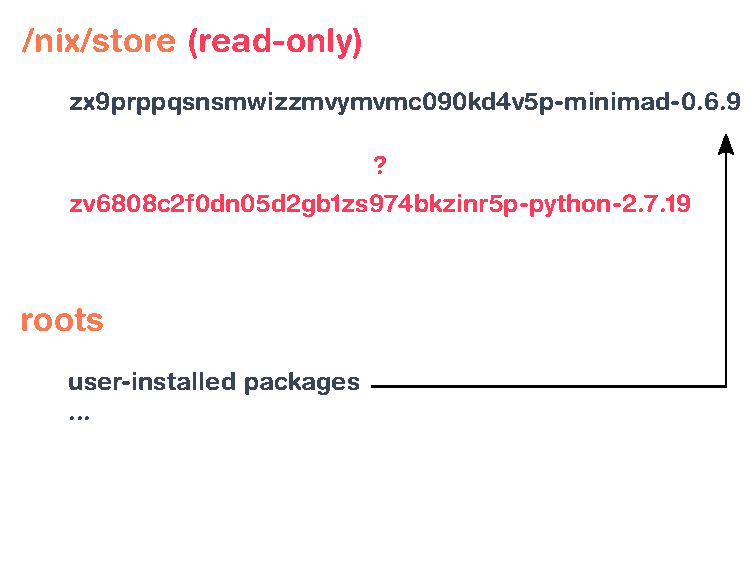
\includegraphics[width=0.95\textwidth]{img/schema-nix-store-gc-3.pdf}
        \end{center}
    }
    \only<9> {
        \begin{center}
            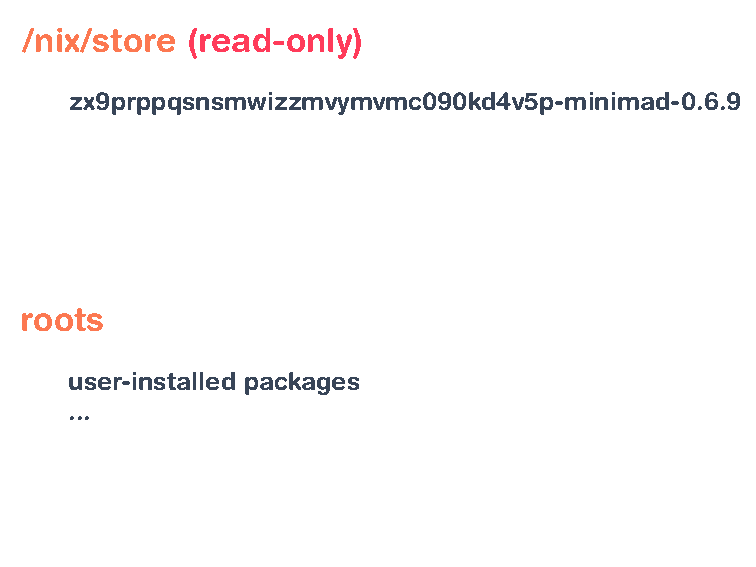
\includegraphics[width=0.95\textwidth]{img/schema-nix-store-gc-4.pdf}
        \end{center}
    }
\end{frame}

\begin{frame}{Perks}
    \begin{block}{Nix}
        \begin{itemize}
            \item Declarative
            \item Reproducible
            \item Complete dependencies
            \item Fearless upgrades: atomic upgrades and rollbacks
        \end{itemize}
    \end{block}
\end{frame}

\begin{frame}{Functional package management}
    \begin{center}
        \begin{tabular}{l|l}
            \couleur{blue-portage}{Nix} &
            \couleur{orange-vivid-tangerine}{Functional programming} \\
            \hline
            Read-only store & Immutability \\
            Hash addressing + sharing & Hash consing \\
            Cleaning & Garbage collection \\
            \couleur{blue-portage}{Reproducibility} &
            \couleur{orange-vivid-tangerine}{Referential transparency} \\
        \end{tabular}
    \end{center}
\end{frame}

\section{Nix expressions}

\begin{frame}
   Building a package should be a \couleur{blue-portage}{pure} function:
   use a functional programming language!
\end{frame}

\begin{frame}{Nix expressions}
\begin{center}
    Nix expressions $=$ \couleur{blue-portage}{JSON} $+$
    \couleur{pink-froly}{$\lambda$}
\end{center}
\end{frame}

\begin{frame}[fragile]{Nix expressions}
\begin{lstlisting}[language=Nix]
{python2WithOpenCV, opencv, stdenv}:
$@stdenv.mkDerivation rec {
  pname = "gh-from-shoe-rust";
  version = "2021-04-30";@$

  buildInputs = [ python2WithOpenCV opencv ];

  $@installPhase = ''
    mkdir -p $out/bin
    cp ${./myscript.py} $out/bin/myscript
  '';
};@$
\end{lstlisting}
\end{frame}

\begin{frame}[fragile]{Derivation: Nix machine code}
\begin{lstlisting}
Derive(
  [("out","/nix/store/qya..-gh-from-shoe","","")],
  [
    ("/nix/store/ae4..-python-2-7-10.drv",
      ["out"]),
    ("/nix/store/78f..-opencv-1-14.drv",
      ["out"]),
    ...
  ["/nix/store/9kr..-default-builder.sh"],
  "x86_64-linux",
  ...
\end{lstlisting}
\end{frame}

\begin{frame}{State of affairs}
    Nix expressions outgrew their initial scope.

    \begin{exampleblock}{In the wild}
      \begin{itemize}
        \item Object systems (kind of): overriding
        \item A module system: NixOS
        \item Non-trivial algorithms (e.g. topological sort)
        \item No types
        \item and so on.
      \end{itemize}
    \end{exampleblock}
\end{frame}

\section{Nickel}

\begin{frame}{Meet Nickel}
    \begin{block}{A new take}
        \begin{itemize}
            \item Gradual typing
            \item Run-time contracts
            \item Recursive records merge system
            \item Stand-alone language (Terraform, Kubernetes, etc.)
        \end{itemize}
    \end{block}
\end{frame}

\begin{frame}[fragile]{A teaser: contract}
\begin{lstlisting}[language=Nickel,title={contracts.ncl}]
let Port = $...$

let Service = {
  name | doc "Service name"
       | Str,

  openPorts | doc "Open ports (firewall)"
            | List #Port
            | default = [],
  $...$
}
\end{lstlisting}
\end{frame}

\begin{frame}[fragile]{A teaser: configuration}
\begin{lstlisting}[language=Nickel,title={nginx.ncl}]
  $let portToUrl : Str -> Num -> Str =
    fun host port => ...  in

  {
    name = "nginx",$
    openPorts = [80, 443],
    $server = "localhost",$
    urls = lists.map
      (portToUrl server)
      openPorts,
  $}$
  | Service
\end{lstlisting}
\end{frame}

\begin{frame}[fragile]{A teaser: result}
\begin{lstlisting}[language=Json,title={nginx.json}]
${
  "name": "nginx",
  "openPorts": [
    80,
    443
  ],
  "server": "localhost",$
  "urls": [
    "http://localhost",
    "https://localhost"
  ]
$}$
\end{lstlisting}
\end{frame}

\begin{frame}[fragile]{Untyped code}
    By default, code is \couleur{pink-froly}{untyped}:
    \begin{itemize}
        \item Terminating \& fixed inputs
        \item JSON interop
        \item Contracts for validation
    \end{itemize}

    \begin{exampleblock}{Example}
\begin{lstlisting}[language=Nickel]
services = [
  "init",
  {name = "firewall", bin = "/bin/firewall"},
  {name = "service", repo = "github.com/johndoe/dns-service"}
]
\end{lstlisting}
    \end{exampleblock}
\end{frame}

\begin{frame}[fragile]{Typed code}
    Library code is \couleur{blue-portage}{statically typed}:
    \begin{itemize}
        \item Triggered by \emph{annotations}
        \item Scoped
        \item Type-inference
    \end{itemize}

\begin{exampleblock}{Example}
   \begin{lstlisting}[language=Nickel]
map : forall a b. (a -> b) -> List a -> List b
    = fun f list =>
  if list == [] then []
  else
    let head = lists.head list in
    let tail = lists.tail list in
    [f head] @ map f tail
\end{lstlisting}
\end{exampleblock}
\end{frame}

\begin{frame}[fragile]{Interaction typed/untyped}

\begin{alertblock}{Problem}
Untyped code can sneak in ill-typed parameters
\end{alertblock}

\vspace{10pt}

\begin{exampleblock}{Example}
\begin{lstlisting}[language=Nickel]
let add : Num -> Num -> Num
        = fun x y => x + y in
add "a" 0
\end{lstlisting}

\begin{lstlisting}[language=Terminal,style=Terminal]
let add : Num -> Num -> Num = fun x y => x + y
                                         ^
This expression has type Str, expected Num
\end{lstlisting}
\end{exampleblock}
\end{frame}

\begin{frame}[fragile]{Contracts, the invisible glue}
Typed code is protected by run-time casts, or \emph{contracts}.

\vspace{10pt}

\begin{lstlisting}[language=Nickel,title={Generated code for \lstinline+add+}]
let safeNum = fun value =>
    if builtins.isNum value then value
    else panic! in

let addSafe = fun x y =>
  let safeX = safeNum x in
  let safeY = safeNum y in
  safeNum (safeX + safeY)
\end{lstlisting}
\end{frame}

\begin{frame}{Contracts, the invisible glue}
  \makebox[\textwidth]{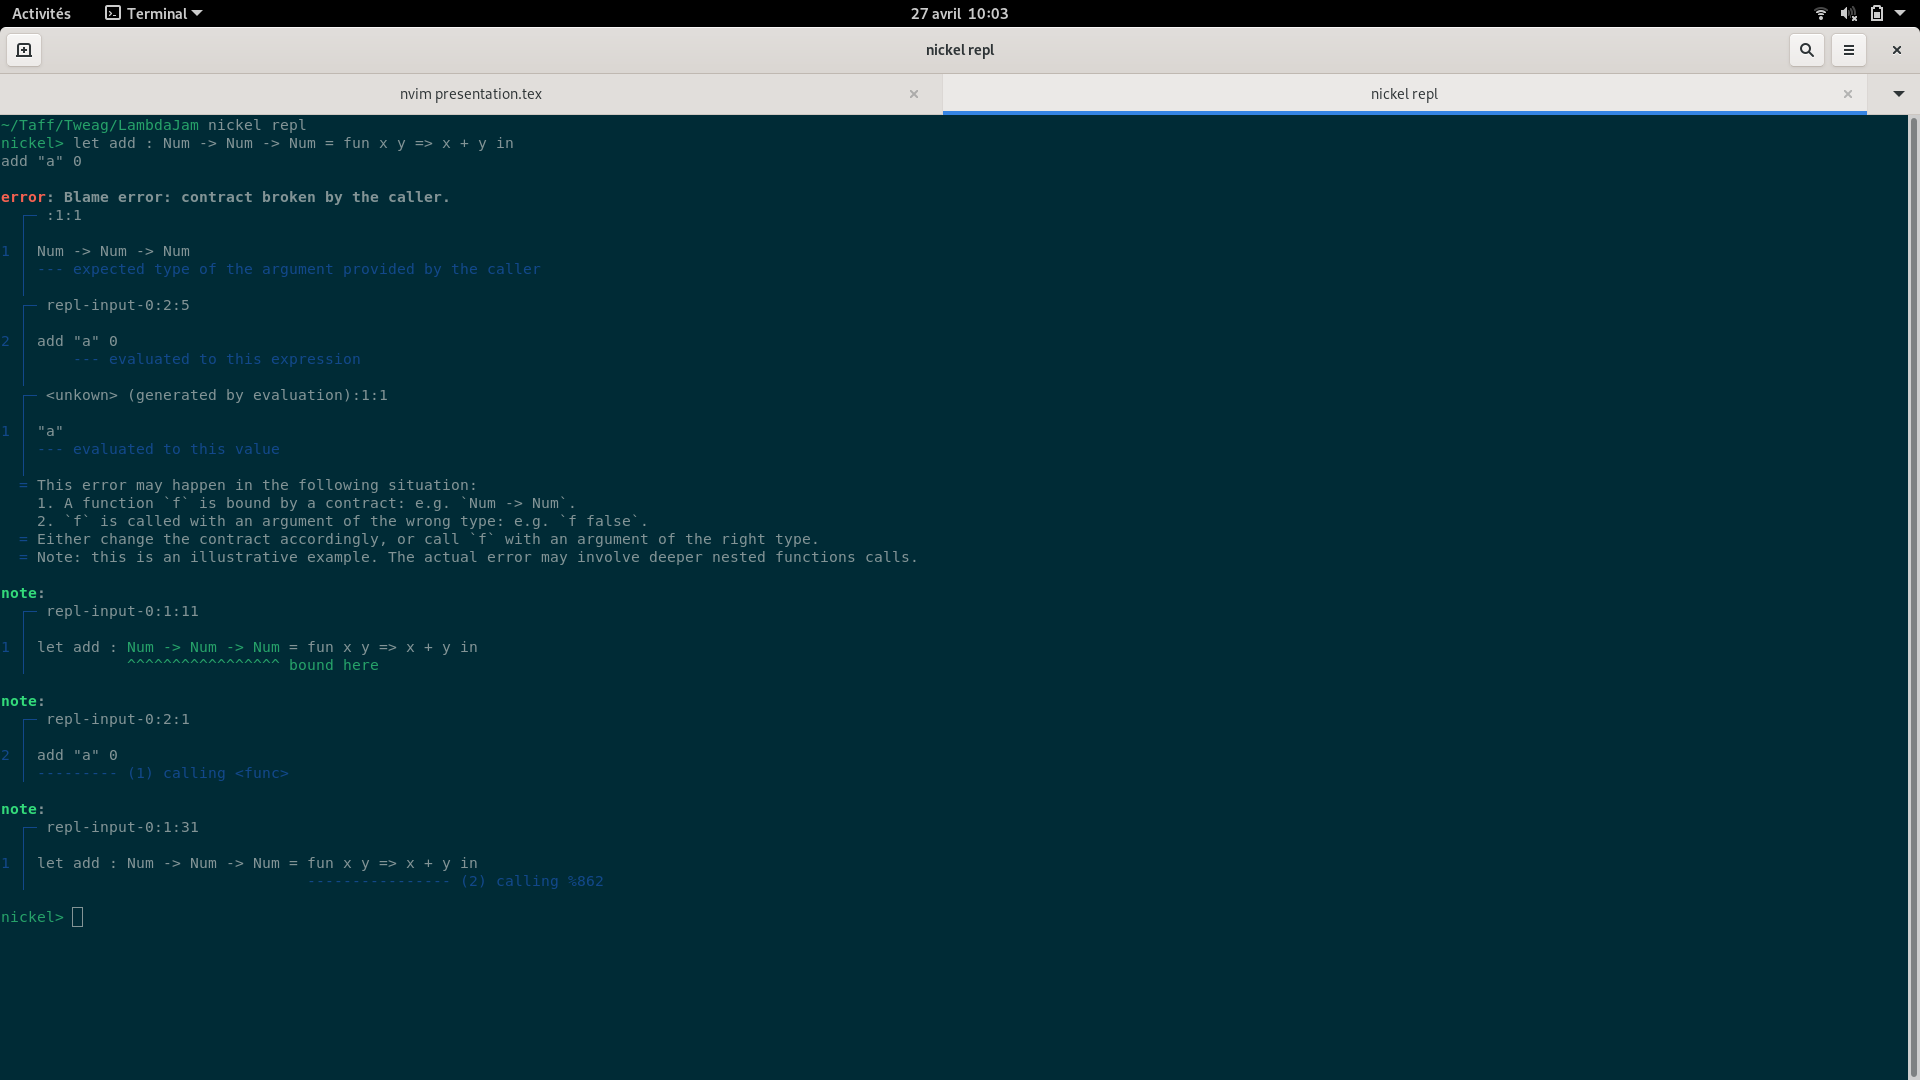
\includegraphics[width=\paperwidth]{img/screen-contract-error.png}}
\end{frame}

\begin{frame}[fragile]{First-class contracts}
\begin{lstlisting}[language=Nickel]
let Url =
  $let pattern = "[-a-zA-Z0-9@:..." in
  fun label value =>
    if builtins.isStr value then
      if strings.isMatch value pattern then
        value
      else
        contracts.blame
          (contracts.tag "invalid URL" label)
    else
      contracts.blame
        (contracts.tag "not a string" label)$ in

let mkUrls
  | {url: #Url, pattern: Str} -> List #Url
  = $...$
\end{lstlisting}
\end{frame}

\begin{frame}[fragile]{First-class contracts}
\begin{lstlisting}[language=Nickel]
Derivation | doc "A Nix package, in Nickel" = {
  name | Str,
  buildInputs | List #NixPackage,
},

NixPackage | doc "Interchange format" = {
  package | Str,
  input | Str
        | default = "nixpkgs",
  _type = "package",
},
\end{lstlisting}
\end{frame}

% \begin{frame}[fragile]{First-class contracts}
% \begin{lstlisting}[language=Nickel]
% let EqMod = fun const base label value =>
%   if builtins.isNum value
%     && value % base == const then
%     value
%   else
%     contracts.blame label in
% let Odd = EqMod 1 2 in
% let Even = EqMod 0 2 in
%
% let doubleOdd | #Odd -> #Even = fun x => 2*x
% \end{lstlisting}
% \end{frame}

\begin{frame}{First-class contracts}
    \begin{exampleblock}{Perks}
        \begin{itemize}
            \item Can check arbitrary properties
            \item Composable
            \item Allow safe typed/untyped interactions
            \item Built-in error reporting
        \end{itemize}
    \end{exampleblock}

    \begin{alertblock}{Limits}
        \begin{itemize}
            \item Run-time cost
            \item Untriggered code paths
        \end{itemize}
    \end{alertblock}
\end{frame}

\section{Conclusion}

\begin{frame}{Summary}
    \begin{itemize}
        \item \couleur{orange-vivid-tangerine}{Reproducibility} is a concrete
            and hard problem: Nix helps.
        \item \couleur{orange-vivid-tangerine}{Functional programming} solves
            a similar problem: let's use the same solutions!
        \item What
        % \item \couleur{orange-vivid-tangerine}{Configuration languages} are
        %     interesting beasts that operate under different constraints. But the solutions developed are
            \emph{broadly} interesting.
    \end{itemize}
    % \begin{block}{Reproducibility}
    %     {Reproducibility is a concrete and hard problem.
    %     It needs a new approach.}
    % \end{block}
    %
    % \begin{block}{Same problem, same solution}
    %     Reproducibility $\Leftrightarrow$ Referential transparency
    % \end{block}
    %
    % \begin{block}{Domain specific language}
    %     Specific constraints: specific language
    % \end{block}
    %
    % \begin{block}{Specific problems, general solutions}
    %     Approaches for solving specific challenges are broadly interesting:
    % \end{block}
\end{frame}

\begin{frame}{CONFLANG21}

    \begin{center}
        \textit{Configuration languages are a worthy area of research.}
    \end{center}

    The 1st Workshop on Configuration Languages

    \begin{description}
        \item[Website] https://2021.splashcon.org/home/conflang-2021
        \item[Deadline] Friday 6 August 2021
        \item[Duration] 1 day
        \item[Event] October 2021, at SPLASH 2021
    \end{description}
\end{frame}

\begin{frame}{Links}
    \begin{description}
        \item[Nickel] https://github.com/tweag/nickel/
        \item[Nix] https://nixos.org/
        \item[Tweag's blog] https://www.tweag.io/blog
    \end{description}

    \begin{block}{Contact}
        \begin{itemize}
        \item yann.hamdaoui@tweag.io
        \item hello@tweag.io
        \end{itemize}
    \end{block}
\end{frame}

\end{document}
